\documentclass{article}
\usepackage{lipsum}
% Language setting
% Replace `english' with e.g. `spanish' to change the document language
\usepackage[english]{babel}
% Set page size and margins
% Replace `letterpaper' with `a4paper' for UK/EU standard size
\usepackage[letterpaper,top=2cm,bottom=2cm,left=3cm,right=3cm,marginparwidth=1.75cm]{geometry}

% Useful packages
\usepackage{amsmath}
\usepackage{graphicx}
\usepackage{subcaption}
\usepackage{wrapfig}
\usepackage{pdfpages}
\usepackage{lipsum}
\usepackage{wrapfig}
% \usepackage[colorlinks=true, allcolors=blue]{hyperref}

\usepackage{color}   %May be necessary if you want to color links
\usepackage{hyperref}
\hypersetup{
    colorlinks=true, %set true if you want colored links
    linktoc=all, 
    linkcolor=blue,
}
\usepackage{cleveref}
% More defined colors
\usepackage[dvipsnames]{xcolor}

% Required package
\usepackage{tikz}
\usetikzlibrary{positioning}

\title{Automate 5G Network Configurations with NVIDIA AI LLM Agents and Kinetica Accelerated Database}
\author{Geralyn Chong}
\begin{document}
\maketitle
\tableofcontents
\section{5G-Slicing-lab Overview}
Kinetica Database powers sub-second analytics and vector search on large amounts of real-time data. PHINE.Tech is a 5G startup to enable and accelerate 5G use cases offering a virtual 5G lab like a lab-as-a-serivce. 

Open Air Interface (OAI) is an open-source software stack. \\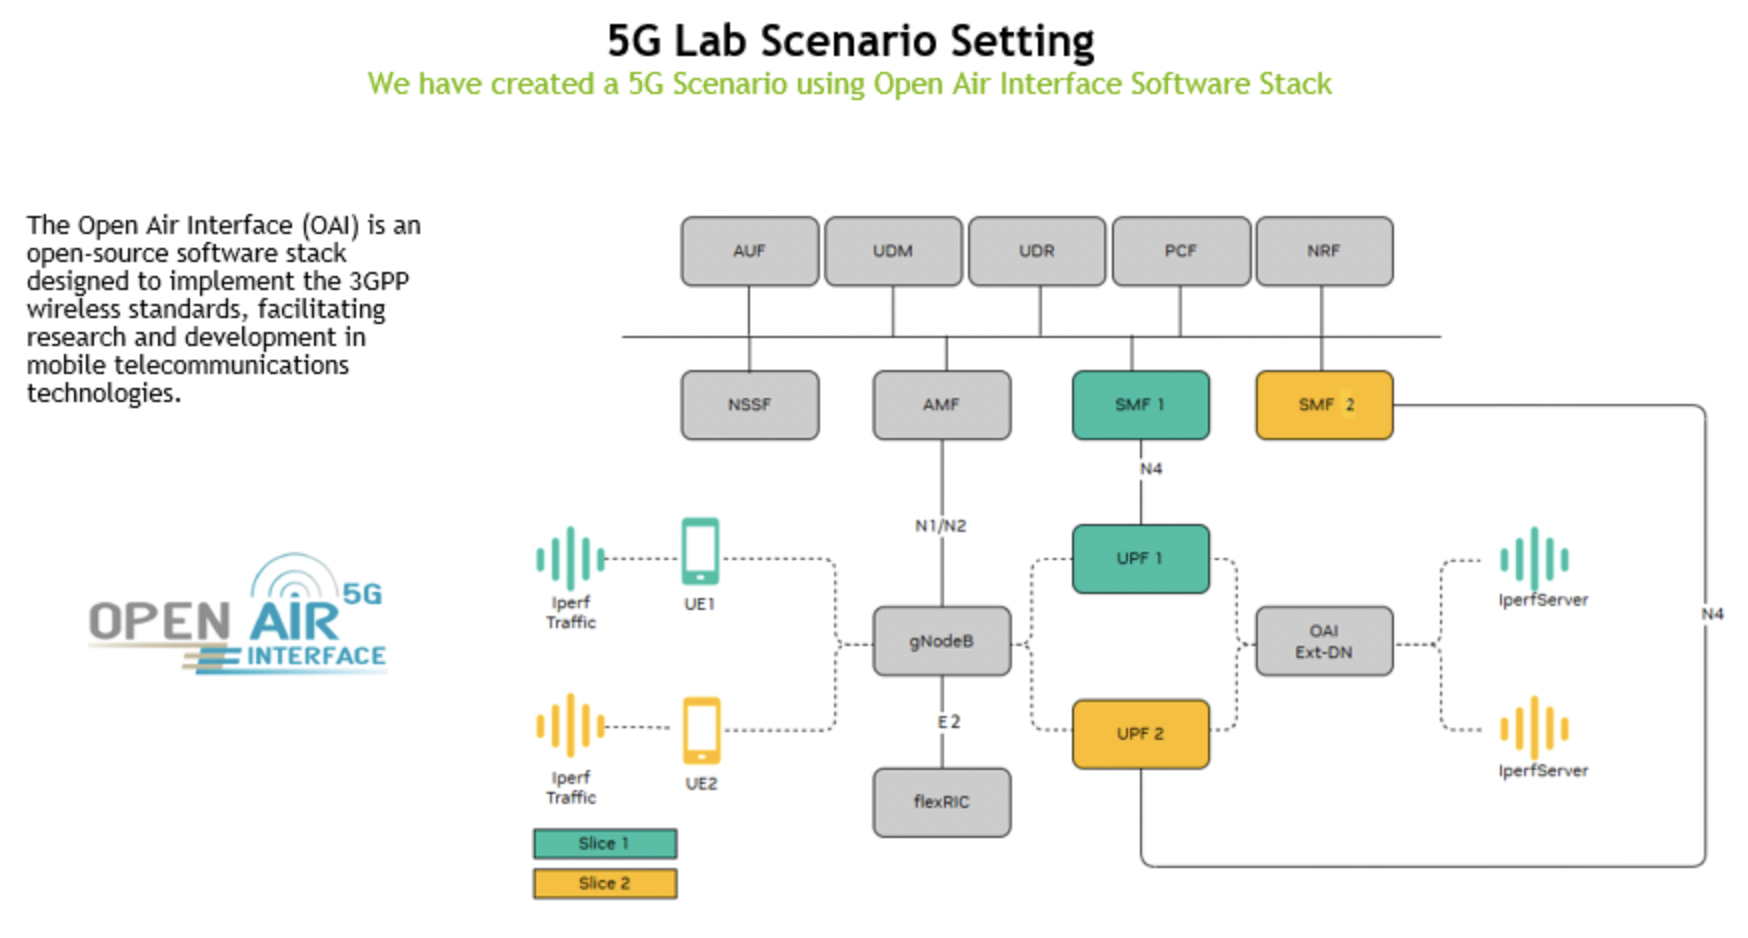
\includegraphics[width=0.9\textwidth]{../images/5glab.png}\\ To simulate traffic that will go through the slices which share the gNodeB. How to configure with an LLM the allocation of slices in the gNodeB (100\% capacity) depending on the traffic generated. 

In the experiment, we include two User Equipments (UEs) across two different network slices, each dynamically adjusting their traffic rate between 30 Mbps and 120 Mbps every 100 milliseconds, with an AI gent dynamically managing slice allocations within the gNodeb. We will have a traffic generator with iPerf to the UE. Each time slot, the UEs are going to push different bit rates. 

\textbf{Location?} This is a very basic setup why do we need an LLM? Idea: We will always have a perception / monitoring mechanism and an action / configuration mechanism in order to execute actions accordingly. 
\section{Introduction to LLM-Agents}
LLM Agents autonomously performing tasks, make decisions, and interact with users or other systems. \begin{itemize}
    \item LLM/Agent Core - Central enginge responsible for understanding and generating text. It defines agent's behavior and serves as the orimary decision-making unit
    \item Planning module - determines the sequence of actions needed to accomplish a goal
    \item Memory Module
    \item Tools - 
\end{itemize}
Orchestration Agent directs the more specialize agents that complete provided tasks broken down from the user / larger problem. 

Agentic Frameworks - structured environments for building AI agents that can reason, plan, and execute tasks autonomously.  Interactions between LLMs, memory, tools, and external environments. \\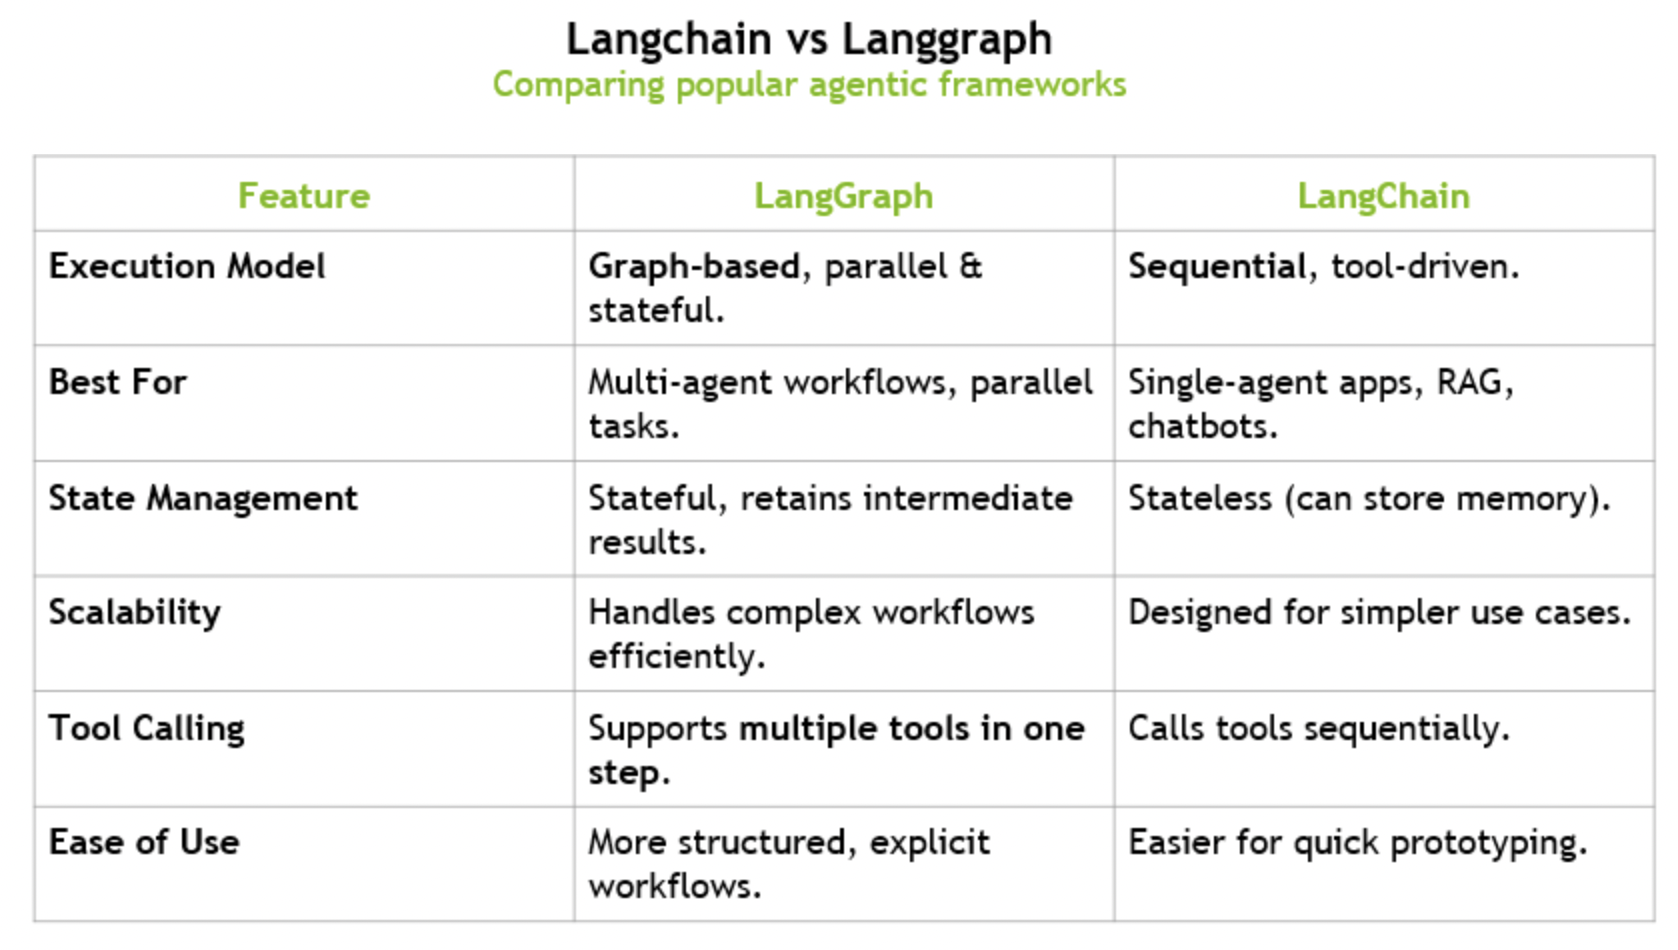
\includegraphics[width=0.8\textwidth]{../images/langChainvsgraph.png}\\
\section{Agent Building Essentials}
Tool Calling allows LLMs to invoke external functions, APIs, or utilities dynamically. 

\subsection{ReAct Agent in Langgraph}
Agent Architecture that combines step-by-step reasoning with tool use. LangGraph provides a prebuilt function \verb|create_react_agent()| 
\section{5G Network Agent Overview}
\subsection{5G-Network Architecture}
We have two agents: Monitoring agent and the network configuration agent. The monitoring takes in the gNobeB logs and parse the logs looking for errors. This error detection calls the network configuration agent which access the \verb|get_pkt_loss_tool| and the \verb|reconfigure_network_tool|. The \verb|get_pkt_loss_tool| is connected to the Kinetica database retrieves the latest packet loss. Analyzing the logs and determines which UE needs more bandwidth. Based on this, it assigns higher bandwidth to the selected UE. This triggers a call to the reconfigure network tool. 


\end{document}